\documentclass{standalone}
\usepackage{tikz}
\begin{document}
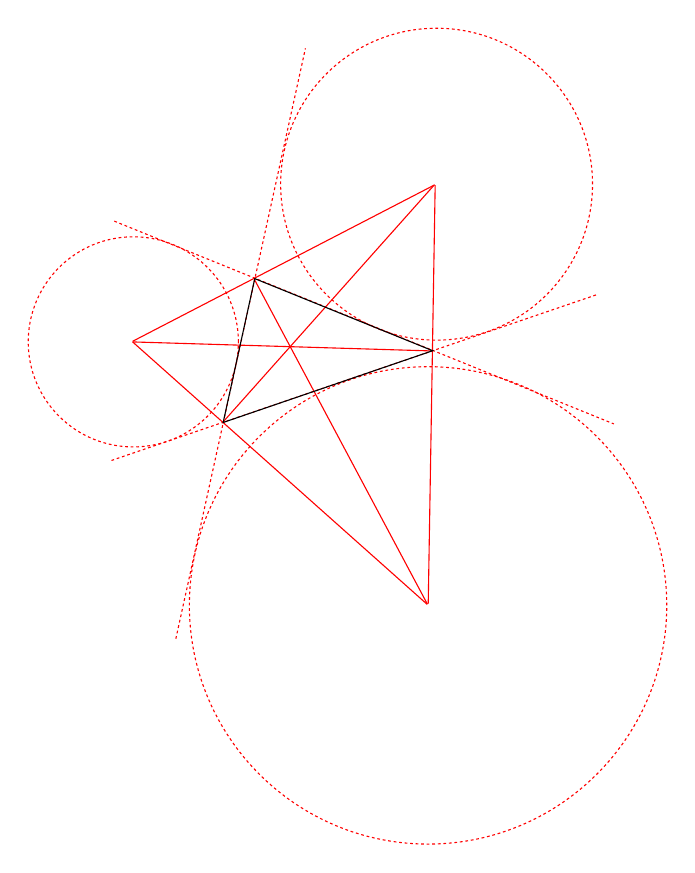
\begin{tikzpicture}[x=1pt,y=1pt]
\draw[red, dash pattern=on 1pt] (41.04,-114.71) circle (37.97);
\draw[red] (73.64,-143.48) -- (149.72,-58.09);
\draw[red] (84.93,-92.39) -- (147.28,-209.43);
\draw[red] (147.61,-209.29) -- (150.12,-58.10);
\draw[red] (148.49,-117.98) -- (40.72,-114.73);
\draw[red] (40.80,-114.73) -- (147.24,-209.57);
\draw[red] (149.96,-57.96) -- (40.84,-114.48);
\draw[red, dash pattern=on 1pt] (34.17,-71.09) -- (214.69,-144.37);
\draw[red, dash pattern=on 1pt] (33.15,-157.56) -- (208.38,-97.71);
\draw[red, dash pattern=on 1pt] (56.41,-221.99) -- (103.24,-8.64);
\draw[red, dash pattern=on 1pt] (150.63,-57.73) circle (56.35);
\draw[red, dash pattern=on 1pt] (147.55,-209.93) circle (86.25);
\draw (84.93,-91.86) -- (73.51,-143.84) -- (149.22,-117.91) -- cycle;
\end{tikzpicture}
\end{document}
